\subsection{Raytracing}
\begin{wrapfigure}{r}{0.3\linewidth}
\centering
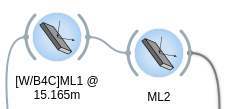
\includegraphics[width=0.3\textwidth]{images/DMM_oasys.png}
\caption{\label{fig:DMM_oasys} Double Multilayer Monochromator in Oasys Shadow.}
\end{wrapfigure}

The double-bounce DMM is modelled with two Shadow Plane Mirror widgets in series (Figure \ref{fig:DMM_oasys}). ML reflectivity is modelled with a Shadow PreMLayer widget as shown in Figure \ref{fig:PreMLayer}. The mirror surface error is is simulated with external splines with varying slope error (0.1, 0.2, 0.25, 0.3, 0.35, 0.4 and 0.5 $\mu rad$ RMS) along the beam axis (Z). Modified surfaces (\ref{fig:fractals}) are generated with the Shadow PreProcessor - Height Profile Simulator widget. The slope error perpendicular to the beam axis (X) is kept constant at 20 $\mu rad$ RMS, and fractal profiles are chosen. 

\begin{figure}  % spans both columns
\begin{subfigure}{0.5\textwidth}
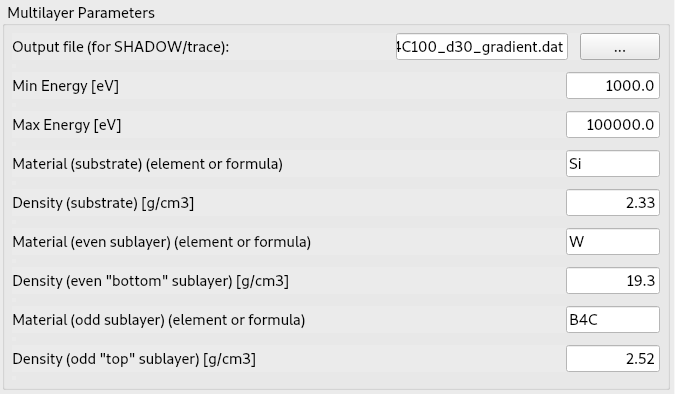
\includegraphics[width=\linewidth]{images/MLspecs_a.png}
\end{subfigure}
\hfill % maximize the horizontal distance between the graphs
\begin{subfigure}{0.5\textwidth}
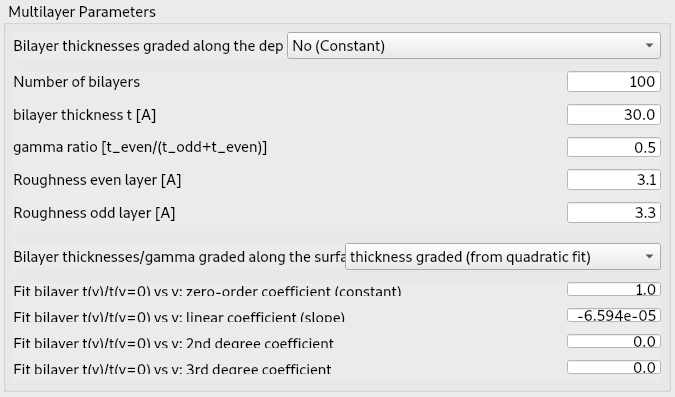
\includegraphics[width=\linewidth]{images/MLspecs_b.png}
\end{subfigure}
\caption{\label{fig:PreMLayer} PreMLayer widget settings in Shadow. }
\end{figure}

\begin{figure}[!htb]
\minipage{0.32\textwidth}
  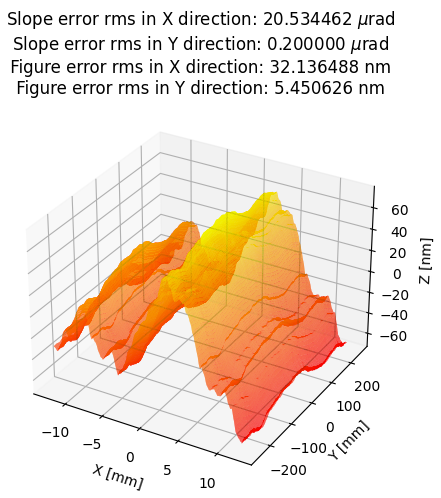
\includegraphics[width=\linewidth]{./../figures/slope_error/surface_error_profile_500x25_02x20urad.png}
  % \caption{A really Awesome Image}\label{fig:awesome_image1}
\endminipage\hfill
\minipage{0.32\textwidth}
  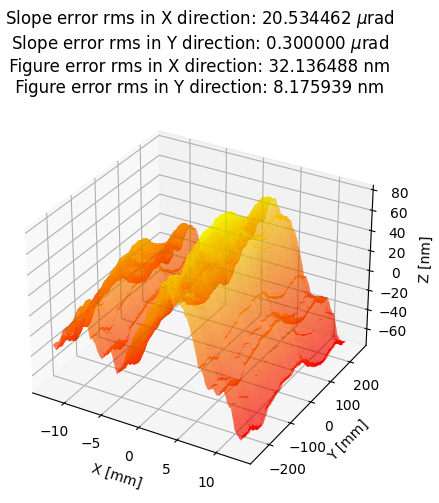
\includegraphics[width=\linewidth]{./../figures/slope_error/surface_error_profile_500x25_03x20urad.png}
  % \caption{A really Awesome Image}\label{fig:awesome_image2}
\endminipage\hfill
\minipage{0.32\textwidth}%
  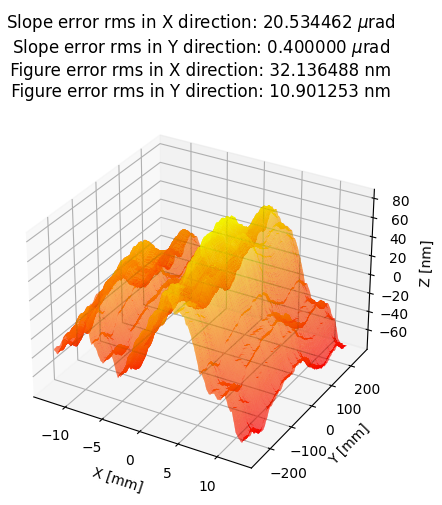
\includegraphics[width=\linewidth]{./../figures/slope_error/surface_error_profile_500x25_04x20urad.png}
  %\caption{A really Awesome Image}\label{fig:awesome_image3}
\endminipage
\caption{\label{fig:fractals} Modified mirror surfaces. In this figure the Y-axis corresponds to the beam path and the X-axis is perpendicular to the beam. }
\end{figure}
